\documentclass[11pt,a4paper]{article}

% ---------- packages ----------
\usepackage[utf8]{inputenc}
\usepackage[T1]{fontenc}
\usepackage[margin=2.2cm]{geometry}
\usepackage{xcolor}
\usepackage{amssymb}
\usepackage{booktabs}
\usepackage{enumitem}
\usepackage{listings}
\usepackage{tikz}
\usetikzlibrary{arrows.meta,positioning,calc,shapes.geometric,backgrounds,fit}
\usepackage[siunitx,RPvoltages]{circuitikz}
\usepackage[colorlinks=true,linkcolor=blue!50!black,urlcolor=blue!50!black]{hyperref}

% ---------- colours ----------
\definecolor{coldblue}{RGB}{30,120,200}
\definecolor{hotred}{RGB}{200,50,40}
\definecolor{metal}{RGB}{150,150,160}
\definecolor{boxblue}{RGB}{225,238,250}
\definecolor{boxgreen}{RGB}{225,245,228}
\definecolor{boxorange}{RGB}{252,237,213}

% ---------- block styles ----------
\tikzset{
  block/.style={draw,rounded corners,minimum width=2.6cm,minimum height=1cm,align=center,font=\small,fill=boxblue},
  sens/.style ={draw,rounded corners,minimum width=2.6cm,minimum height=1cm,align=center,font=\small,fill=boxgreen},
  pwr/.style  ={draw,rounded corners,minimum width=2.6cm,minimum height=1cm,align=center,font=\small,fill=boxorange},
  flow/.style ={-{Latex[length=2.5mm]},thick},
  lbl/.style  ={font=\scriptsize,fill=white,inner sep=1pt,align=center}
}

% ---------- code style ----------
\lstdefinestyle{ino}{
  language=C++,
  basicstyle=\ttfamily\footnotesize,
  keywordstyle=\color{blue!70!black}\bfseries,
  commentstyle=\color{green!45!black}\itshape,
  stringstyle=\color{red!60!black},
  numbers=left,numberstyle=\tiny\color{gray},numbersep=7pt,
  breaklines=true,frame=single,framesep=4pt,rulecolor=\color{gray!50},
  showstringspaces=false,tabsize=2,
  morekeywords={IRAM_ATTR,ledcAttach,ledcWrite,digitalRead,digitalWrite,pinMode,
    attachInterrupt,digitalPinToInterrupt,Serial,INPUT_PULLUP,OUTPUT,HIGH,LOW,
    RISING,millis,delay}
}

% ---------- helper boxes ----------
\newcommand{\yes}{\textcolor{green!50!black}{\checkmark}}
\newcommand{\warn}{\textcolor{orange!80!black}{$\triangle$}}
\newcommand{\no}{\textcolor{red!70!black}{$\times$}}
\newsavebox{\gbbox}
\newenvironment{checkbox}[1]
  {\par\medskip\noindent\begin{lrbox}{\gbbox}\begin{minipage}{0.95\linewidth}\footnotesize\textbf{#1}\par\smallskip}
  {\end{minipage}\end{lrbox}\setlength{\fboxsep}{8pt}\fcolorbox{red!60!black}{red!5}{\usebox{\gbbox}}\par\medskip}
\newenvironment{tipbox}[1]
  {\par\medskip\noindent\begin{lrbox}{\gbbox}\begin{minipage}{0.95\linewidth}\footnotesize\textbf{#1}\par\smallskip}
  {\end{minipage}\end{lrbox}\setlength{\fboxsep}{8pt}\fcolorbox{green!45!black}{green!5}{\usebox{\gbbox}}\par\medskip}

\title{\vspace{-1.5cm}\textbf{Build Guide for Beginners}\\[3pt]
\large How to build the moving cart for the solar-panel cleaning robot ---\\[2pt]
\large explained from zero, one small step at a time}
\author{Graduation Project --- prototype phase}
\date{17 June 2026}

\begin{document}
\maketitle
\vspace{-0.5cm}

\noindent\fbox{\parbox{0.98\linewidth}{\small
\textbf{Read this first.} This guide assumes you have never wired electronics or built a frame before.
Every word that might be new is explained the first time it appears. Do the steps \textbf{in order}. Do
not skip the safety page. If something does not work, look for the red \warn\ ``If it goes wrong'' box
right under that step.}}

\tableofcontents

% ============================================================
\section{What you are building, in one minute}

Your final robot will ride along a solar panel, make its own water from the air using small cooling
chips, and wash the dust off. That is too much to build at once. So we build it in pieces.

\textbf{This guide builds the first piece: the moving cart.} It is a little trolley that slides along a
metal track by itself, drives to one end, then comes back, over and over. That is the same motion the
real robot uses to sweep a panel. Once the cart moves on its own, you have proven the hardest mechanical
part works. The water-making part is added later, when the remaining parts arrive.

\begin{tipbox}{Why we start here}
You already own every part needed for the moving cart. You do \emph{not} yet own the parts for the
water-making chips (big heatsinks and a strong power supply). So we build what is possible now and get a
real, working result this week.
\end{tipbox}

% ============================================================
\section{Meet your parts --- what each piece looks like}

Before wiring anything, learn to recognise each part by sight. People often mix these up. In particular:

\begin{checkbox}{\warn\ The red board is NOT the motor}
The flat red board with the blue screw blocks (the one you photographed, marked ``HW-095'') is the
\textbf{L298N driver} --- the ``muscle.'' It has \emph{no} shaft. The \textbf{motor} is a separate part:
a small silver cylinder with a short metal rod (the shaft) at one end and a bundle of wires at the other.
The pulley goes on that rod, never on the red board.
\end{checkbox}

\subsection*{The motor (GA25-370) --- where the shaft is}

\begin{figure}[h]
\centering
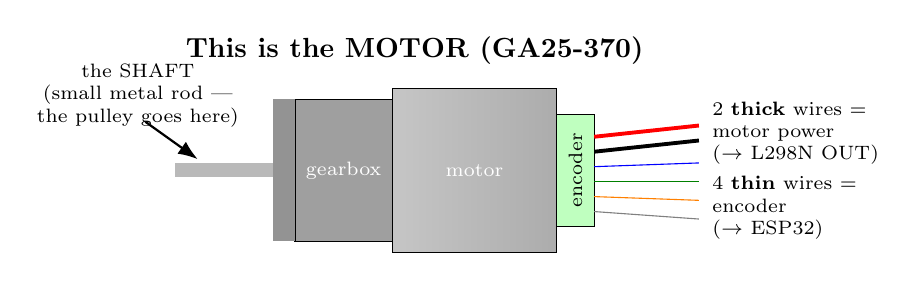
\begin{tikzpicture}[scale=0.95]
% motor body
\shade[left color=gray!45,right color=gray!65] (4.2,0) rectangle (6.4,2.2);
\draw (4.2,0) rectangle (6.4,2.2);
% gearbox
\fill[gray!75] (2.9,0.15) rectangle (4.2,2.05);
\draw (2.9,0.15) rectangle (4.2,2.05);
\node[font=\scriptsize,white] at (3.55,1.1){gearbox};
% front plate
\fill[gray!85] (2.6,0.15) rectangle (2.9,2.05);
% shaft
\draw[line width=5pt,gray!55] (2.6,1.1)--(1.3,1.1);
\node[font=\scriptsize,align=center] at (0.8,2.1){the SHAFT\\(small metal rod ---\\the pulley goes here)};
\draw[flow] (0.9,1.75)--(1.6,1.25);
% body label
\node[font=\scriptsize,white] at (5.3,1.1){motor};
% encoder
\fill[green!25] (6.4,0.35) rectangle (6.9,1.85);
\draw (6.4,0.35) rectangle (6.9,1.85);
\node[font=\scriptsize,align=center,rotate=90] at (6.65,1.1){encoder};
% wires
\draw[red,line width=1.4pt] (6.9,1.55)--(8.3,1.7);
\draw[black,line width=1.4pt] (6.9,1.35)--(8.3,1.5);
\draw[blue] (6.9,1.15)--(8.3,1.2);
\draw[green!50!black] (6.9,0.95)--(8.3,0.95);
\draw[orange] (6.9,0.75)--(8.3,0.7);
\draw[gray] (6.9,0.55)--(8.3,0.45);
\node[font=\scriptsize,align=left,right] at (8.35,1.6){2 \textbf{thick} wires =\\motor power\\($\to$ L298N OUT)};
\node[font=\scriptsize,align=left,right] at (8.35,0.6){4 \textbf{thin} wires =\\encoder\\($\to$ ESP32)};
\node[font=\bfseries] at (4.5,2.7){This is the MOTOR (GA25-370)};
\end{tikzpicture}
\caption{The real motor. The shaft is the short rod at the front --- that is the only place a pulley
attaches. The thick pair of wires carries motor power; the four thin wires are the encoder.}
\end{figure}

\subsection*{How the pulley fixes to the shaft}

You do not glue or nail anything. The pulley has a hole through its middle; you slide that hole over the
shaft, then tighten a tiny screw (a ``grub screw'') on the side of the pulley so it grips the rod.

\begin{figure}[h]
\centering
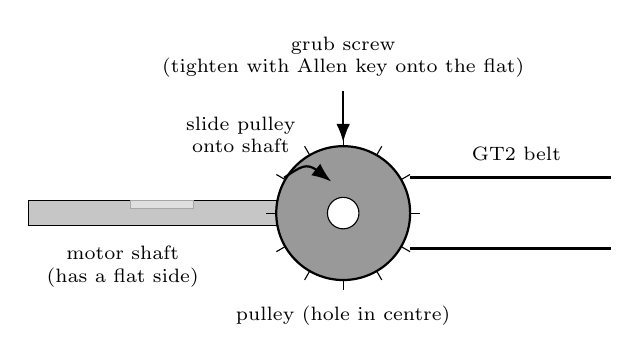
\begin{tikzpicture}[scale=1]
% shaft
\fill[gray!45] (0,-0.16) rectangle (3.2,0.16);
\draw (0,-0.16) rectangle (3.2,0.16);
\draw[gray!70,fill=gray!25] (1.3,0.06) rectangle (2.1,0.16); % flat
\node[below,font=\scriptsize,align=center] at (1.2,-0.3){motor shaft\\(has a flat side)};
% pulley
\draw[thick,fill=gray!80] (4.0,0) circle (0.85);
\foreach \a in {0,30,...,330}{\draw (4.0,0)++(\a:0.85)--++(\a:0.13);}
\draw[fill=white] (4.0,0) circle (0.2);
\node[below,font=\scriptsize] at (4.0,-1.05){pulley (hole in centre)};
% grub screw
\draw[-{Latex},thick] (4.0,1.55)--(4.0,0.9);
\node[above,font=\scriptsize,align=center] at (4.0,1.6){grub screw\\(tighten with Allen key onto the flat)};
% slide arrow
\draw[flow] (3.25,0.45) .. controls (3.55,0.65) .. (3.85,0.4);
\node[font=\scriptsize,align=center] at (2.7,1.0){slide pulley\\onto shaft};
% belt
\draw[very thick] (4.85,0.45)--(7.4,0.45);
\draw[very thick] (4.85,-0.45)--(7.4,-0.45);
\node[font=\scriptsize] at (6.2,0.75){GT2 belt};
\end{tikzpicture}
\caption{The pulley slides onto the shaft and is locked by its grub screw. Aim the screw at the flat part
of the shaft so it cannot spin loose. The belt then wraps around the pulley.}
\end{figure}

\subsection*{The L298N driver (the board you photographed)}

\begin{figure}[h]
\centering
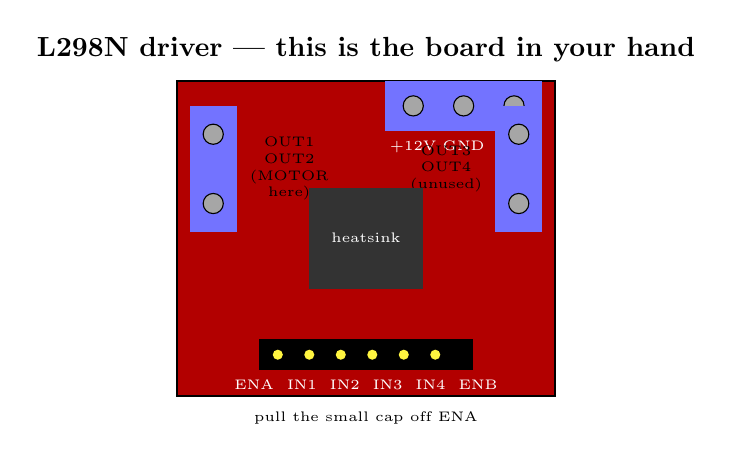
\begin{tikzpicture}[scale=0.8]
\fill[red!70!black] (0,0) rectangle (6,5);
\draw[thick] (0,0) rectangle (6,5);
% power 3-term (top)
\fill[blue!55] (3.3,4.2) rectangle (5.8,5.0);
\foreach \x/\t in {3.75/+12V,4.55/GND,5.35/+5V}{\draw[fill=gray!70] (\x,4.6) circle (0.16); \node[font=\tiny,white,below] at (\x,4.2){\t};}
% motor A (left edge)
\fill[blue!55] (0.2,2.6) rectangle (0.95,4.6);
\foreach \y in {3.05,4.15}{\draw[fill=gray!70](0.575,\y) circle (0.16);}
\node[font=\tiny,align=center,right] at (1.0,3.6){OUT1\\OUT2\\(MOTOR\\here)};
% motor B (right edge, unused)
\fill[blue!55] (5.05,2.6) rectangle (5.8,4.6);
\foreach \y in {3.05,4.15}{\draw[fill=gray!70](5.425,\y) circle (0.16);}
\node[font=\tiny,align=center,left] at (5.0,3.6){OUT3\\OUT4\\(unused)};
% heatsink
\fill[black!80] (2.1,1.7) rectangle (3.9,3.3);
\node[font=\tiny,white] at (3.0,2.5){heatsink};
% logic header (bottom)
\fill[black] (1.3,0.4) rectangle (4.7,0.9);
\foreach \x in {1.6,2.1,...,4.4}{\fill[yellow!75](\x,0.65) circle (0.08);}
\node[font=\tiny,white,below] at (3.0,0.4){ENA \ IN1 \ IN2 \ IN3 \ IN4 \ ENB};
\node[font=\tiny,align=center] at (3.0,-0.35){pull the small cap off ENA};
\node[font=\bfseries,align=center] at (3.0,5.5){L298N driver --- this is the board in your hand};
\end{tikzpicture}
\caption{The L298N. Motor's two thick wires go to OUT1/OUT2 (left block). The 12\,V adapter goes to the
top block (+12V, GND). Three thin wires from the ESP32 go to the ENA/IN1/IN2 pins along the bottom.
Remove the little jumper cap sitting on ENA.}
\end{figure}

\subsection*{The other small parts}

\begin{figure}[h]
\centering
\begin{minipage}{0.46\linewidth}\centering
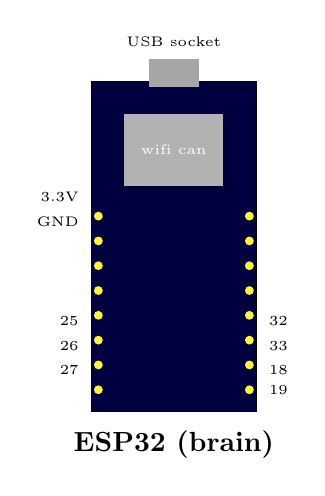
\begin{tikzpicture}[scale=0.7]
\fill[blue!25!black] (0,0) rectangle (3,6); \draw (0,0) rectangle (3,6);
\fill[gray!70] (1.05,5.9) rectangle (1.95,6.4); \node[font=\tiny,above] at (1.5,6.45){USB socket};
\fill[gray!60] (0.6,4.1) rectangle (2.4,5.4); \node[font=\tiny,white] at (1.5,4.75){wifi can};
\foreach \y in {0.4,0.85,...,3.9}{\fill[yellow!80](0.13,\y) circle (0.08);\fill[yellow!80](2.87,\y) circle (0.08);}
\node[font=\tiny,left] at (-0.05,3.9){3.3V};\node[font=\tiny,left] at (-0.05,3.45){GND};
\node[font=\tiny,left] at (-0.05,1.65){25};\node[font=\tiny,left] at (-0.05,1.2){26};\node[font=\tiny,left] at (-0.05,0.75){27};
\node[font=\tiny,right] at (3.05,1.65){32};\node[font=\tiny,right] at (3.05,1.2){33};
\node[font=\tiny,right] at (3.05,0.75){18};\node[font=\tiny,right] at (3.05,0.4){19};
\node[font=\bfseries,align=center] at (1.5,-0.6){ESP32 (brain)};
\end{tikzpicture}
\end{minipage}\hfill
\begin{minipage}{0.46\linewidth}\centering
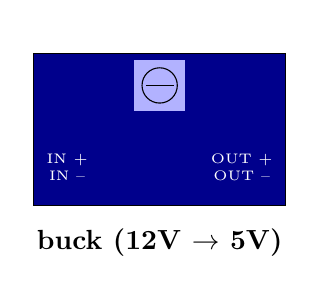
\begin{tikzpicture}[scale=0.8]
\fill[blue!55!black] (0,0) rectangle (4,2.4); \draw (0,0) rectangle (4,2.4);
\fill[blue!30] (1.6,1.5) rectangle (2.4,2.3); \draw (2.0,1.9) circle (0.28); \draw (1.78,1.9)--(2.22,1.9);
\node[font=\tiny,white,above] at (2.0,2.32){set-voltage screw};
\node[font=\tiny,white,align=center,right] at (0.05,0.6){IN +\\IN --};
\node[font=\tiny,white,align=center,left] at (3.95,0.6){OUT +\\OUT --};
\node[font=\bfseries,align=center] at (2,-0.6){buck (12V $\to$ 5V)};
\end{tikzpicture}
\par\vspace{0.7cm}
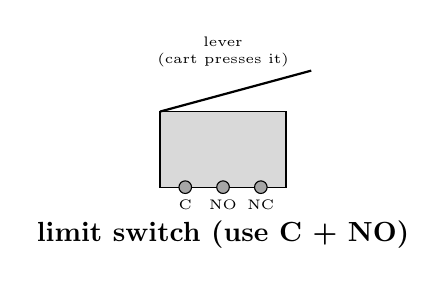
\begin{tikzpicture}[scale=0.8]
\fill[gray!30] (0,0) rectangle (2,1.2); \draw (0,0) rectangle (2,1.2);
\draw[thick] (0,1.2)--(2.4,1.85);
\node[font=\tiny,align=center] at (1.0,2.15){lever\\(cart presses it)};
\foreach \x/\t in {0.4/C,1.0/NO,1.6/NC}{\draw[fill=gray!70](\x,0) circle (0.1);\node[font=\tiny,below] at (\x,-0.05){\t};}
\node[font=\bfseries,align=center] at (1.0,-0.75){limit switch (use C + NO)};
\end{tikzpicture}
\end{minipage}
\caption{Left: the ESP32 brain --- the pin numbers are printed next to each pin on the real board (exact
positions vary, so read your own board). Right top: the buck converter that makes 5\,V. Right bottom: a
limit switch; wire the C and NO tabs.}
\end{figure}

\noindent The four \textbf{cooling chips (TEC1-12706)} are flat white ceramic squares, each with a red and
a black wire. You met them already; they get marked and stacked in Section~7.

% ============================================================

% ============================================================
\section{Words you will see (plain meanings)}

\begin{description}[leftmargin=2.2cm,style=nextline,itemsep=2pt]
  \item[V-slot rail] A straight aluminium bar with grooves down its sides, like a tiny train rail. The
  cart's wheels sit in the grooves. \textbf{You now have two of these bars.}
  \item[Gantry plate / cart] A flat metal plate with wheels already attached (the OpenBuilds kit). This
  is the trolley that rolls along the rail.
  \item[GT2 belt] A black rubber belt with teeth on one side, like a tiny car timing belt. Pulling the
  belt drags the cart along.
  \item[Pulley] A small toothed wheel the belt wraps around. One pulley sits on the motor; turning it
  moves the belt.
  \item[Idler] A free-spinning pulley at the far end that just guides the belt around the turn.
  \item[Motor (GA25-370)] The small electric motor that spins the pulley. Yours also has an
  \textbf{encoder}.
  \item[Encoder] A tiny sensor built into the back of the motor that counts how much the motor has
  turned, so the computer knows where the cart is.
  \item[ESP32] A small blue circuit board, the ``brain.'' It runs the program you upload and tells the
  motor what to do. It has many metal pins along its edges.
  \item[Pin / GPIO] One of those metal legs on the ESP32. Each has a number (like \texttt{GPIO25}). A
  wire clipped to a pin carries a signal.
  \item[L298N] A red circuit board, the ``muscle.'' The ESP32 is too weak to power a motor directly, so
  it tells the L298N, and the L298N feeds the real power to the motor.
  \item[Driver] General word for that muscle board (the L298N is a motor driver).
  \item[PWM] A trick to control speed: the power is switched on and off very fast; more ``on'' time means
  faster. You do not wire anything special for it --- the program does it.
  \item[Limit switch] A small click button at each end of the rail. When the cart bumps it, the brain
  knows it reached the end and turns the cart around.
  \item[Buck converter (DC-DC step-down)] A little board that turns 12\,volts into 5\,volts, because the
  brain wants 5\,V while the motor wants 12\,V.
  \item[TEC / Peltier tile] A flat square chip (yours are TEC1-12706). When you feed it electricity one
  face gets cold and the other gets hot. The cold face is where water will form later.
  \item[Heatsink] A finned metal block that carries heat away, like the cooler on a computer chip.
  \item[Multimeter] A cheap measuring tool with two probe wires; it tells you voltage and whether two
  points are connected. Very handy. Buy one if you can (about 150 EGP).
\end{description}

% ============================================================
\section{Things to gather before you start}

\textbf{From the parts you already bought:} the 2 V-slot rails, one gantry plate with wheels, the GT2
belt, the 2 pulleys + idler kit, the GA25-370 motor, the ESP32, the red L298N board, the little 12$\to$5
buck board, the 2 limit switches, the M5 T-nuts, and the L-brackets.

\textbf{Still to get for the twin-rail layout you chose:} a \textbf{second gantry plate with wheels} (rides
rail~2) and a \textbf{cross-beam} to join the two plates (a short 2020/2040 extrusion, ~30--40\,cm, or a
stiff flat aluminium bar). You can build and test on rail~1 alone while you wait for these.

\textbf{Small things to grab from home or a hardware shop (cheap):}
\begin{itemize}[leftmargin=*,itemsep=1pt]
  \item A small \textbf{screwdriver set} (a flat one and a Phillips/cross one).
  \item A set of \textbf{Allen keys} (hex keys) --- the OpenBuilds wheels use them.
  \item \textbf{Jumper wires}, the ``male-to-female'' kind (these let you connect boards without
  soldering). A pack is very cheap.
  \item A small \textbf{breadboard} (a white plastic block with holes) --- optional but makes joining
  grounds easy with no soldering.
  \item A \textbf{12\,V power adapter} that can give at least 2--3 amps. A spare router, CCTV, or laptop
  brick that says ``Output: 12V'' on the label works. (The big 24-amp supply is only for the water chips
  later --- not needed now.)
  \item A \textbf{USB cable} that fits the ESP32 (usually micro-USB or USB-C) and \emph{carries data}, not
  a charge-only cable.
  \item A \textbf{permanent marker}, a \textbf{ruler}, and a flat board or table to mount the rail on.
  \item A computer with internet (to install the free Arduino program).
\end{itemize}

% ============================================================
\section{Stay safe (please read)}

\begin{itemize}[leftmargin=*,itemsep=2pt]
  \item \textbf{Never} power a cooling chip (TEC) at full 12\,V unless a heatsink is pressed onto its hot
  side. Without it, the chip destroys itself in under a minute. The quick test in Section~6 uses only
  3--5\,V for a few seconds, which is safe.
  \item Always \textbf{unplug the 12\,V} before you change any wire. Plug in only after you have
  double-checked.
  \item Keep \textbf{water away} from the boards while testing the motion. Water comes later.
  \item Plug the 12\,V adapter into the \textbf{wall last}, and pull it out \textbf{first} when finishing.
  \item If anything smells hot, gets very hot to touch, or smokes --- \textbf{unplug immediately}.
\end{itemize}

% ============================================================
\section{Step group A --- build the track and the cart}

You chose the \textbf{twin-rail} layout: the cart spans \textbf{two parallel rails}, with one gantry
plate riding each rail, exactly like the real robot. This is the most stable version and matches the
deployment design. Only \textbf{one} rail is \emph{driven} by the belt; the other rail's plate just rolls
along to keep the cart square and steady.

\begin{checkbox}{\warn\ You're not blocked while you decide}
Mount the motor, belt and your one gantry plate on \textbf{rail~1 alone} and run the whole motion test
(Sections~10--12) on that single rail first. The \textbf{rail-2 side} is added afterwards --- and there
are \textbf{two ways} to build it, compared right after the diagram below.
\end{checkbox}

\begin{figure}[h]
\centering
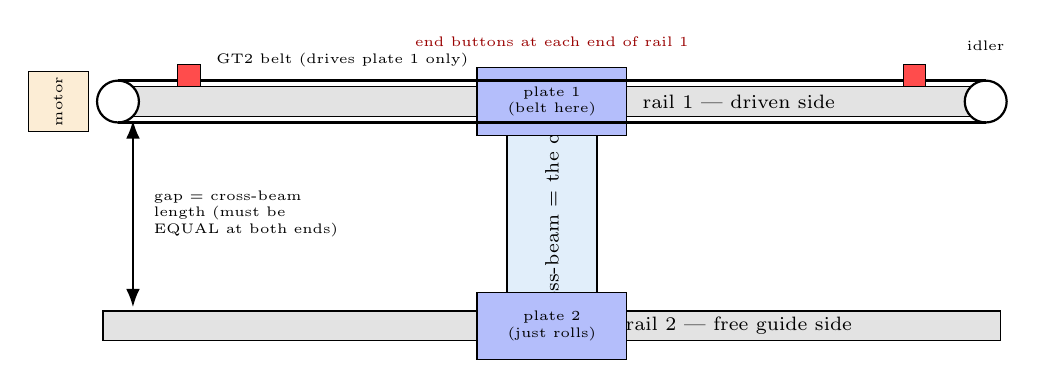
\begin{tikzpicture}[scale=0.95]
% rail 1 (driven)
\fill[gray!22] (0,2.8) rectangle (12,3.2); \draw (0,2.8) rectangle (12,3.2);
\node[font=\scriptsize] at (8.5,3.0){rail 1 --- driven side};
% rail 2 (free)
\fill[gray!22] (0,-0.2) rectangle (12,0.2); \draw (0,-0.2) rectangle (12,0.2);
\node[font=\scriptsize] at (8.5,0.0){rail 2 --- free guide side};
% cross-beam
\fill[boxblue] (5.4,0) rectangle (6.6,3.0); \draw[thick] (5.4,0) rectangle (6.6,3.0);
\node[font=\scriptsize,align=center,rotate=90] at (6.0,1.5){cross-beam = the cart};
% gantry plates
\fill[boxblue!80!blue] (5.0,2.55) rectangle (7.0,3.45); \draw (5.0,2.55) rectangle (7.0,3.45);
\node[font=\tiny,align=center] at (6.0,3.0){plate 1\\(belt here)};
\fill[boxblue!80!blue] (5.0,-0.45) rectangle (7.0,0.45); \draw (5.0,-0.45) rectangle (7.0,0.45);
\node[font=\tiny,align=center] at (6.0,0.0){plate 2\\(just rolls)};
% motor + pulley
\fill[boxorange] (-1.0,2.6) rectangle (-0.2,3.4); \draw (-1.0,2.6) rectangle (-0.2,3.4);
\node[font=\tiny,align=center,rotate=90] at (-0.6,3.0){motor};
\draw[thick,fill=white] (0.2,3) circle (0.28);
\draw[thick,fill=white] (11.8,3) circle (0.28);
\node[font=\tiny] at (11.8,3.75){idler};
% belt
\draw[very thick] (0.2,3.28)--(11.8,3.28);
\draw[very thick] (0.2,2.72)--(11.8,2.72);
\node[font=\tiny,fill=white,inner sep=1pt] at (3.2,3.55){GT2 belt (drives plate 1 only)};
% limit switches
\draw[fill=red!70] (1.0,3.2) rectangle (1.3,3.5);
\draw[fill=red!70] (10.7,3.2) rectangle (11.0,3.5);
\node[font=\tiny,red!60!black] at (6.0,3.8){end buttons at each end of rail 1};
% gap arrow
\draw[{Latex}-{Latex},thick] (0.4,0.25)--(0.4,2.75);
\node[font=\tiny,align=left,right] at (0.55,1.5){gap = cross-beam\\length (must be\\EQUAL at both ends)};
\end{tikzpicture}
\caption{Twin-rail layout, from above. Two parallel rails; the cart is a cross-beam riding a gantry plate
on each rail. Only rail~1 is driven by the belt; rail~2's plate rolls along to keep the cart square. The
rails must stay exactly parallel --- measure the gap at both ends.}
\end{figure}

\subsection*{Building the rail-2 side --- two ways}

Rail~1 carries your existing gantry plate plus the belt and motor. The \textbf{rail-2} side only has to
roll along and keep the cart square, so you can either build it yourself or buy a matching plate. Both
give the same cart-spans-two-rails result.

\begin{center}\small
\begin{tabular}{@{}p{2.6cm}p{5.7cm}p{5.7cm}@{}}
\toprule
 & \textbf{Option A --- DIY rail-2 bogie} & \textbf{Option B --- buy a 2nd gantry plate} \\
\midrule
What you add & 2--4 V-wheels on a small bracket/plate + a cross-beam & OpenBuilds 2nd mini gantry plate (with wheels) + a cross-beam \\
Extra cost & \textasciitilde 390--580 EGP (2--4 wheels @\textasciitilde 95 + \textasciitilde 200 beam; bracket from parts on hand) & \textasciitilde 590 EGP (390 plate + \textasciitilde 200 beam) \\
Effort & more hands-on: drill the bracket, set the wheel spacing to the rail & bolt-together, parts already matched \\
Sturdiness & good if the bracket is rigid & best (precise, matched) \\
Real-robot look & yes & yes \\
Pick it if & you want to save a little and don't mind DIY & you want the cleanest build, no fiddling \\
\bottomrule
\end{tabular}
\end{center}

\begin{figure}[h]
\centering
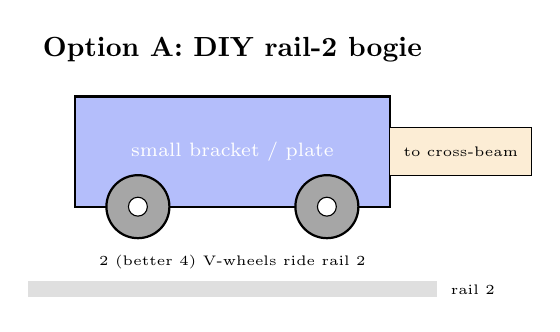
\begin{tikzpicture}[scale=1]
% bracket plate
\fill[boxblue!80!blue] (0,0) rectangle (4,1.4); \draw[thick] (0,0) rectangle (4,1.4);
\node[font=\scriptsize,white] at (2,0.7){small bracket / plate};
% wheels
\draw[thick,fill=gray!70] (0.8,0) circle (0.4); \draw[fill=white](0.8,0) circle (0.12);
\draw[thick,fill=gray!70] (3.2,0) circle (0.4); \draw[fill=white](3.2,0) circle (0.12);
\node[font=\tiny,align=center] at (2.0,-0.7){2 (better 4) V-wheels ride rail 2};
% rail 2
\fill[gray!25] (-0.6,-1.15) rectangle (4.6,-0.95); \node[font=\tiny,right] at (4.65,-1.05){rail 2};
% cross-beam stub
\fill[boxorange] (4,0.4) rectangle (5.8,1.0); \draw (4,0.4) rectangle (5.8,1.0);
\node[font=\tiny] at (4.9,0.7){to cross-beam};
\node[font=\bfseries] at (2,2.0){Option A: DIY rail-2 bogie};
\end{tikzpicture}
\caption{Option A: a couple of V-wheels on a small bracket make the rail-2 side; the cross-beam bolts this
bogie to your plate on rail~1. Option B simply swaps this home-made bogie for a second ready-made gantry
plate --- everything else is identical.}
\end{figure}

\begin{enumerate}[leftmargin=*,itemsep=3pt]
  \item \textbf{Lay both rails parallel} on your flat board --- same direction, same height, a fixed gap
  apart. The gap must equal the length of your cross-beam. Screw each rail down with L-brackets + M5
  T-nuts (a T-nut slides into the groove, the L-bracket sits on top, a bolt clamps them).
  \item \textbf{Make them truly parallel.} Measure the gap between the two rails at the left end and again
  at the right end --- the two numbers must match. If they differ, the cart will jam. Nudge a rail until
  the gap is equal at both ends.
  \item \textbf{Put the rolling parts on each rail.} Your existing plate goes on rail~1. On rail~2 put
  either your DIY V-wheel bogie (Option~A) or a bought gantry plate (Option~B). Slide each on so its
  V-wheels sit in the grooves like a drawer.
  \item \textbf{Adjust the wheels} on each plate: turn the \textbf{eccentric nut} (an off-centre nut that
  tightens the wheel) until that plate rolls smoothly with no wobble and no looseness.
  \item \textbf{Bolt the cross-beam across both plates} with corner brackets + T-nuts. This joins the two
  plates into one cart. Push it by hand --- both plates must glide together with no binding. If it jams,
  the rails are not parallel: go back to step~2.
  \item \textbf{Fix the motor} at the left end of \textbf{rail~1} (the driven rail), shaft pointing along
  the rail. Use the round motor bracket, or clamp the motor body to an L-bracket for now.
  \item \textbf{Push a pulley onto the motor shaft} and tighten its tiny side screw (grub screw) so it
  grips the flat of the shaft and cannot spin loose.
\end{enumerate}

\begin{checkbox}{\warn\ If it goes wrong --- the pulley is loose on the motor shaft}
Your pulleys have a 5\,mm hole, but the motor's shaft is a bit smaller (about 4\,mm with a flat side).
Measure both with a ruler. If the pulley is loose: wrap the shaft with a turn of thin tape, or fit a
small sleeve, or aim the grub screw at the flat part of the shaft so it bites. \textbf{If the pulley does
not grip the shaft, the motor will spin but the cart will not move} --- this is the most common beginner
problem, so fix it now.
\end{checkbox}

\begin{enumerate}[leftmargin=*,itemsep=3pt,start=8]
  \item Fix the \textbf{idler} pulley at the far end of \textbf{rail~1}, at the same height as the motor
  pulley, so the belt runs level.
  \item Run the \textbf{belt} along rail~1: clip one end to the cart (the rail-1 side), stretch it down to
  the idler, around it, back to the motor pulley, around that, and clip the other end back to the cart.
  The toothed side must mesh with both pulleys.
  \item Pull the belt \textbf{snug} --- firm, no droop --- but the pulleys must still turn freely by hand.
  \item Put a \textbf{limit switch} at each end, positioned so the cart presses the button just before it
  would run off the rail. Most switches have three metal tabs labelled C (or COM), NO, and NC; we use
  \textbf{C and NO}.
\end{enumerate}

\subsection*{How to fix the idler (the far-end pulley) --- step 8 in detail}

The idler is the pulley at the end \emph{opposite} the motor. It has no power and no grub screw: it just
spins freely on a bolt and does two jobs --- it turns the belt around at the end, and it lets you set the
belt tension. Yours is the ``smooth idler pulley kit.''

\begin{figure}[h]
\centering
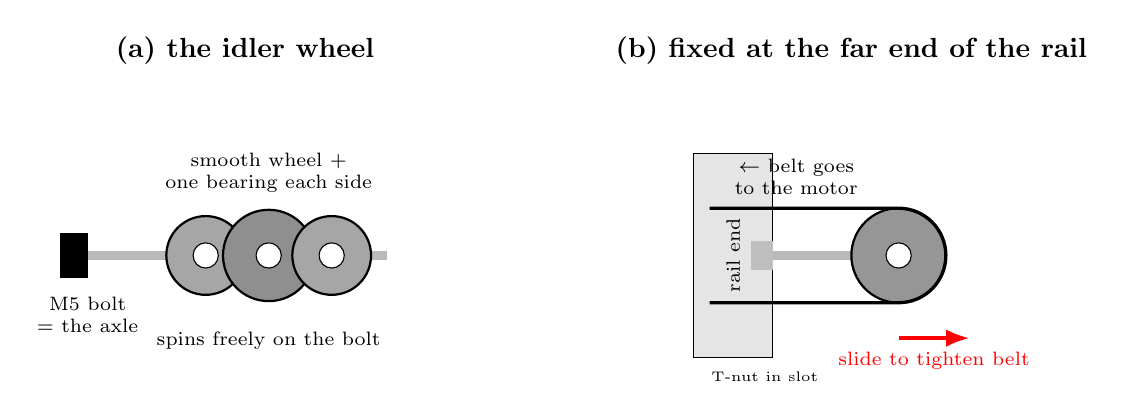
\begin{tikzpicture}[scale=1]
% ---- (a) exploded idler ----
\begin{scope}
\node[font=\bfseries] at (1.8,2.6){(a) the idler wheel};
% bolt axle
\draw[line width=3pt,gray!55] (-0.2,0)--(3.6,0);
\fill[black] (-0.55,-0.28) rectangle (-0.2,0.28);
\node[font=\scriptsize,align=center,below] at (-0.2,-0.4){M5 bolt\\= the axle};
% bearing 1
\draw[thick,fill=gray!70] (1.3,0) circle (0.5); \draw[fill=white](1.3,0) circle (0.16);
% idler wheel
\draw[thick,fill=gray!88] (2.1,0) circle (0.58); \draw[fill=white](2.1,0) circle (0.16);
% bearing 2
\draw[thick,fill=gray!70] (2.9,0) circle (0.5); \draw[fill=white](2.9,0) circle (0.16);
\node[font=\scriptsize,align=center] at (2.1,1.05){smooth wheel +\\one bearing each side};
\node[font=\scriptsize,below] at (2.1,-0.85){spins freely on the bolt};
\end{scope}
% ---- (b) mounted at far end ----
\begin{scope}[xshift=7.5cm]
\node[font=\bfseries] at (2.0,2.6){(b) fixed at the far end of the rail};
% rail end
\fill[gray!20] (0,-1.3) rectangle (1.0,1.3); \draw (0,-1.3) rectangle (1.0,1.3);
\node[font=\scriptsize,rotate=90] at (0.5,0){rail end};
% T-nut
\fill[gray!50] (0.72,-0.18) rectangle (1.0,0.18);
\node[font=\tiny,align=center,below] at (0.9,-1.35){T-nut in slot};
% bolt
\draw[line width=3pt,gray!55] (1.0,0)--(2.6,0);
% idler
\draw[thick,fill=gray!82] (2.6,0) circle (0.6); \draw[fill=white](2.6,0) circle (0.16);
% belt wrap (right half) + lines back toward motor
\draw[very thick] (0.2,0.6)--(2.6,0.6) arc (90:-90:0.6) -- (0.2,-0.6);
\node[font=\scriptsize,align=center] at (1.3,1.0){$\leftarrow$ belt goes\\to the motor};
% tension arrow
\draw[-{Latex},very thick,red] (2.6,-1.05)--(3.5,-1.05);
\node[font=\scriptsize,red,below] at (3.05,-1.1){slide to tighten belt};
\end{scope}
\end{tikzpicture}
\caption{The idler: two bearings inside a smooth wheel, spinning on a bolt (a). Mounted at the far end on
a T-nut, with the belt wrapping its outer side; sliding it away from the motor tightens the belt (b).}
\end{figure}

\begin{enumerate}[leftmargin=*,itemsep=3pt]
  \item If your idler came as loose pieces, build the wheel first: press one bearing into each side of the
  smooth wheel with the thin shim between them. If it is already one wheel that spins, skip this.
  \item Push an \textbf{M5 bolt} through the centre hole --- this bolt is the idler's axle.
  \item Drop a \textbf{T-nut} into the slot at the \textbf{far end} of the rail (the end with no motor).
  Pass the bolt through the idler and screw it into the T-nut (or through a hole in an end L-bracket).
  \textbf{Do not fully tighten yet.}
  \item Set the idler at the \textbf{same height} as the motor pulley and in a \textbf{straight line} with
  it, so the belt runs level and straight --- not slanted across.
  \item Wrap the belt around the idler. Then slide the whole idler a little \emph{away} from the motor to
  pull the belt tight, and now tighten its bolt to lock it in that spot.
  \item Check: the belt is firm with no droop, the idler spins freely when you flick it, and the belt
  teeth sit in the middle of both pulleys without rubbing the edges.
\end{enumerate}

\begin{tipbox}{The idler is your tension knob}
Whenever the belt goes loose later, you do not rebuild anything --- just loosen the idler bolt, slide the
idler a touch further from the motor, and retighten. That is the normal way to tension a belt.
\end{tipbox}

\begin{checkbox}{\warn\ If the belt climbs off or rubs one edge}
The idler is not level with the motor pulley, or the two are not lined up straight. Loosen the idler bolt,
move it so both pulleys are at the same height and directly in line, then retighten. A crooked idler makes
the belt walk sideways and jump off.
\end{checkbox}

\begin{tipbox}{Quick check before electronics}
With no power at all, push the cart by hand from one end to the other. It should glide smoothly and click
each end button. If it drags or wobbles, fix the wheels (step 4) before going further. Mechanics first,
electricity second.
\end{tipbox}

% ============================================================
\section{Step group B --- find the cold side of each cooling chip}

You will not power the chips for water yet, but label them now so they are ready. You asked how to tell
which side is hot and which is cold --- here is the simple, safe way.

\begin{figure}[h]
\centering
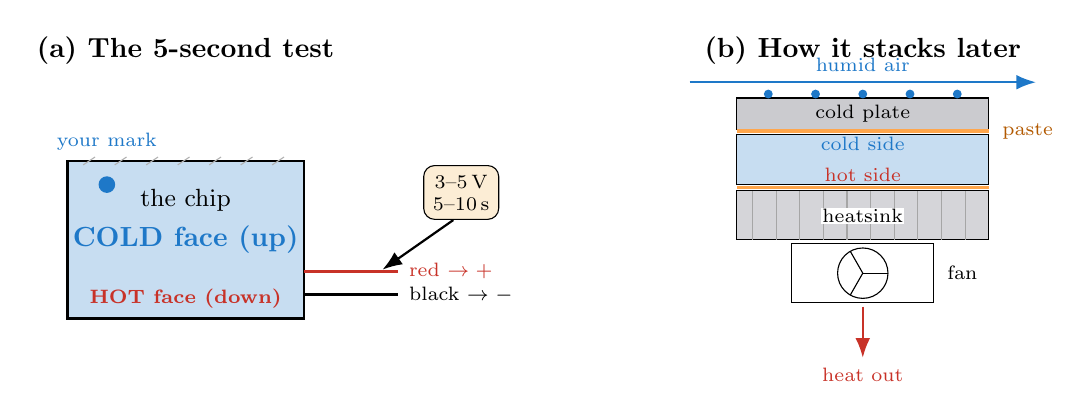
\begin{tikzpicture}
% ---- (a) the test ----
\begin{scope}[xshift=0cm]
  \node[font=\bfseries] at (1.5,3.4) {(a) The 5-second test};
  \fill[coldblue!25] (0,0) rectangle (3,2);
  \draw[thick] (0,0) rectangle (3,2);
  \foreach \x in {0.2,0.6,...,2.8}{\draw[gray!60] (\x,1.95)--(\x+0.15,2.05);}
  \node at (1.5,1.5) {\small the chip};
  \node[coldblue,font=\bfseries] at (1.5,1.0) {COLD face (up)};
  \node[hotred,font=\bfseries\scriptsize] at (1.5,0.25) {HOT face (down)};
  \draw[hotred,very thick] (3,0.6) -- (4.2,0.6) node[right,font=\scriptsize]{red $\to +$};
  \draw[black,very thick]  (3,0.3) -- (4.2,0.3) node[right,font=\scriptsize]{black $\to -$};
  \node[draw,rounded corners,fill=boxorange,font=\scriptsize,align=center] at (5.0,1.6)
    {3--5\,V\\5--10\,s};
  \draw[flow] (4.9,1.25) -- (4.0,0.62);
  \fill[coldblue] (0.5,1.7) circle (3pt);
  \node[font=\scriptsize,coldblue] at (0.5,2.25){your mark};
\end{scope}
% ---- (b) the stack ----
\begin{scope}[xshift=8.5cm]
  \node[font=\bfseries] at (1.6,3.4) {(b) How it stacks later};
  \draw[flow,coldblue] (-0.6,3.0) -- (3.8,3.0) node[midway,above,font=\scriptsize]{humid air};
  \fill[metal!50] (0,2.4) rectangle (3.2,2.8);
  \draw (0,2.4) rectangle (3.2,2.8); \node[font=\scriptsize] at (1.6,2.6){cold plate};
  \foreach \x in {0.4,1.0,1.6,2.2,2.8}{\fill[coldblue] (\x,2.85) circle (1.6pt);}
  \draw[orange!70,very thick] (0,2.38)--(3.2,2.38); \node[orange!70!black,font=\scriptsize,right] at (3.25,2.38){paste};
  \fill[coldblue!25] (0,1.7) rectangle (3.2,2.34);
  \draw (0,1.7) rectangle (3.2,2.34);
  \node[coldblue,font=\scriptsize] at (1.6,2.22){cold side};
  \node[hotred,font=\scriptsize] at (1.6,1.82){hot side};
  \draw[orange!70,very thick] (0,1.66)--(3.2,1.66);
  \fill[metal!40] (0,1.0) rectangle (3.2,1.62);
  \draw (0,1.0) rectangle (3.2,1.62);
  \foreach \x in {0.2,0.5,...,3.0}{\draw[gray!70] (\x,1.0)--(\x,1.62);}
  \node[font=\scriptsize,fill=white,inner sep=0.5pt] at (1.6,1.3){heatsink};
  \draw (0.7,0.2) rectangle (2.5,0.95);
  \draw (1.6,0.575) circle (0.32);
  \draw (1.6,0.575)--++(0.32,0); \draw (1.6,0.575)--++(-0.16,0.28);\draw(1.6,0.575)--++(-0.16,-0.28);
  \node[font=\scriptsize,right] at (2.55,0.575){fan};
  \draw[flow,hotred] (1.6,0.15) -- (1.6,-0.5) node[below,font=\scriptsize]{heat out};
\end{scope}
\end{tikzpicture}
\caption{Left: the safe little test that tells you which face is cold. Right: the order things will be
stacked later --- water forms on the cold plate; the hot side must touch a heatsink and fan.}
\end{figure}

\begin{enumerate}[leftmargin=*,itemsep=2pt]
  \item Set your power source to a \textbf{low voltage: 3 to 5\,V} (a couple of AA batteries in a holder
  is perfect; \textbf{do not use 12\,V} for this test). Lay one chip flat with nothing pressed on it.
  \item Touch the chip's \textbf{red} wire to $+$ and the \textbf{black} wire to $-$ for only
  \textbf{5--10 seconds}. One face quickly turns clearly cold to the finger.
  \item With your marker, put a dot on the \textbf{cold} face. That is the side that will face the water
  plate later.
  \item If the face you expected to be cold came out hot instead, just swap the two wires. Keep all four
  chips marked the same way.
\end{enumerate}

\begin{checkbox}{\warn\ Important}
This brief 3--5\,V test is the \emph{only} time you may run a chip without a heatsink, and only for a few
seconds. Do not connect 12\,V to a bare chip.
\end{checkbox}

% ============================================================
\section{Step group C --- connect the electronics}

We will connect three boards: the \textbf{ESP32} (brain), the \textbf{L298N} (muscle), and the
\textbf{buck converter} (the 12$\to$5\,V helper). Use the male-to-female jumper wires --- one end pushes
onto a board's pin, the other end screws into the L298N's little terminals or pushes onto its pins.

\begin{figure}[h]
\centering
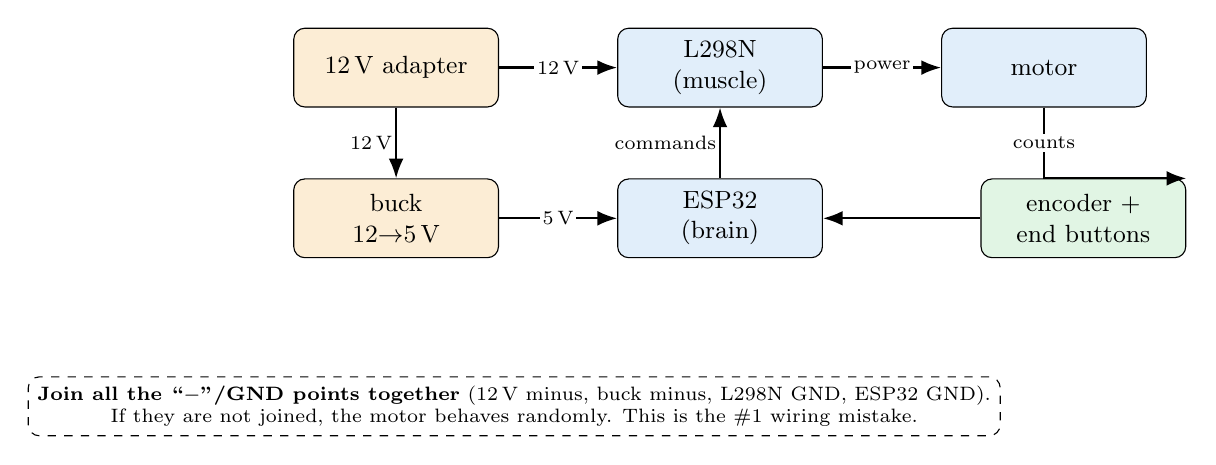
\begin{tikzpicture}[node distance=0.9cm and 1.5cm]
\node[pwr] (src) {12\,V adapter};
\node[block,right=of src] (l298) {L298N\\(muscle)};
\node[block,right=of l298] (mot) {motor};
\node[pwr,below=of src] (buck) {buck\\12$\to$5\,V};
\node[block,below=of l298] (esp) {ESP32\\(brain)};
\node[sens,right=2.0cm of esp] (sens) {encoder +\\end buttons};
\draw[flow] (src) -- node[lbl]{12\,V} (l298);
\draw[flow] (l298) -- node[lbl]{power} (mot);
\draw[flow] (src) -- node[lbl,left]{12\,V} (buck);
\draw[flow] (buck) -- node[lbl]{5\,V} (esp);
\draw[flow] (esp) -- node[lbl,left]{commands} (l298);
\draw[flow] (mot.south) |- node[lbl,pos=0.25]{counts} (sens.north east);
\draw[flow] (sens) -- (esp);
\node[font=\scriptsize,align=center,draw,dashed,rounded corners,below=1.5cm of buck.south,xshift=1.5cm]
  (gnd){\textbf{Join all the ``$-$''/GND points together} (12\,V minus, buck minus, L298N GND, ESP32 GND).\\
  If they are not joined, the motor behaves randomly. This is the \#1 wiring mistake.};
\end{tikzpicture}
\caption{The big picture. The 12\,V adapter feeds the muscle board and the buck; the buck makes 5\,V for
the brain; the brain sends commands to the muscle, which powers the motor.}
\end{figure}

\noindent\textbf{Do the connections in this order. Keep the 12\,V unplugged while wiring.}

\begin{enumerate}[leftmargin=*,itemsep=3pt]
  \item \textbf{Motor to muscle.} The motor's two \emph{thick} wires (the pair that spins it) screw into
  the L298N terminals marked \textbf{OUT1} and \textbf{OUT2}.
  \item \textbf{Power into the muscle.} The 12\,V adapter's $+$ goes to the L298N \textbf{+12V} terminal;
  its $-$ goes to the L298N \textbf{GND} terminal. Do not plug into the wall yet.
  \item \textbf{Make 5\,V.} Wire the same 12\,V into the buck converter's \textbf{IN} ($+$ and $-$). The
  buck's \textbf{OUT} gives 5\,V --- send that to the ESP32's \textbf{5V (or VIN)} pin and \textbf{GND}.
  \item \textbf{Brain to muscle (the commands).} Use three jumper wires from the ESP32 to the L298N:
  \begin{center}\small
  \begin{tabular}{@{}lll@{}}
  \toprule
  ESP32 pin & L298N pin & what it does\\
  \midrule
  GPIO25 & ENA & speed\\
  GPIO26 & IN1 & one direction\\
  GPIO27 & IN2 & other direction\\
  \bottomrule
  \end{tabular}
  \end{center}
  On the L298N, \textbf{pull off the small jumper cap on ENA} so your speed control works (with the cap
  on, the motor only runs full speed).
  \item \textbf{Encoder (the counter) to the brain.} The motor's four \emph{thin} wires are the encoder:
  \begin{center}\small
  \begin{tabular}{@{}ll@{}}
  \toprule
  Encoder wire (colours vary --- check your seller) & Connect to\\
  \midrule
  Vcc (often blue) & ESP32 \textbf{3V3} pin (not 5\,V)\\
  GND (often green) & ESP32 GND\\
  signal A (often yellow) & ESP32 GPIO32\\
  signal B (often white, thin) & ESP32 GPIO33\\
  \bottomrule
  \end{tabular}
  \end{center}
  \item \textbf{End buttons to the brain.} Left button: one tab to ESP32 \textbf{GPIO18}, the other tab to
  GND. Right button: one tab to \textbf{GPIO19}, the other to GND.
  \item \textbf{Join all grounds.} Make sure every ``$-$''/GND mentioned above meets at one common point
  (a breadboard ground row makes this easy). Re-read the dashed note in the figure.
\end{enumerate}

\begin{tipbox}{How to tell motor wires from encoder wires}
The two wires that make the motor spin when you briefly touch them to a single AA battery are the
\emph{thick} motor pair. The other four thin wires are the encoder. Never put the motor's thick wires
into the ESP32 --- they go only to the L298N.
\end{tipbox}

% ============================================================
\section{Step group D --- put the program on the brain}

The ESP32 does nothing until you load a program (called a ``sketch''). Here is how, from zero.

\begin{enumerate}[leftmargin=*,itemsep=3pt]
  \item On your computer, open a browser, go to \texttt{arduino.cc}, download \textbf{Arduino IDE}, and
  install it (keep clicking Next/Agree).
  \item Open Arduino IDE. Click \textbf{File $\to$ Preferences}. In the box ``Additional boards manager
  URLs'', paste:\\
  \texttt{https://espressif.github.io/arduino-esp32/package\_esp32\_index.json}\\ then click OK.
  \item Click \textbf{Tools $\to$ Board $\to$ Boards Manager}. Type \texttt{esp32}. Install
  ``\textbf{esp32 by Espressif}'' (this downloads the ESP32 support; wait for it to finish).
  \item Plug the ESP32 into the computer with the USB \emph{data} cable.
  \item Click \textbf{Tools $\to$ Board $\to$ esp32 $\to$ ESP32 Dev Module}.
  \item Click \textbf{Tools $\to$ Port} and pick the new port that appeared (something like
  \texttt{COM5}).
  \item Open the file \texttt{bench\_motion.ino.txt} (next to this guide), copy its text into a new
  Arduino sketch. The exact program is printed below so you can check it.
  \item Click the round \textbf{Upload} button (the right-arrow at top-left). Wait until it says
  ``\textbf{Done uploading}.''
  \item Click \textbf{Tools $\to$ Serial Monitor}, set the speed box to \textbf{115200}. You will see
  lines of numbers --- that is the brain reporting the cart's direction and position count.
\end{enumerate}

\begin{checkbox}{\warn\ If upload fails or no port appears}
The USB cable may be charge-only (try another), or the driver for the ESP32's USB chip is missing. Look
at the small chip near the USB socket: if it says \textbf{CP2102}, install the ``CP210x'' driver; if
\textbf{CH340}, install the ``CH340'' driver (both are free, search the chip name). Some ESP32 boards
need you to \emph{hold the BOOT button} while the upload starts.
\end{checkbox}

\noindent The program (already saved as \texttt{bench\_motion.ino.txt}):
\lstinputlisting[style=ino]{bench_motion.ino.txt}

% ============================================================
\section{Step group E --- first power-up and test}

\begin{enumerate}[leftmargin=*,itemsep=3pt]
  \item Leave the ESP32 plugged into the computer by USB (this powers the brain and shows the numbers).
  \item Double-check every wire against Section~8. Especially: grounds joined, motor wires in OUT1/OUT2,
  ENA jumper cap removed.
  \item Now plug the \textbf{12\,V adapter into the wall}. The cart should start driving toward one end.
  \item When it reaches an end and presses the button, it should stop, pause, and go back the other way,
  repeating forever.
\end{enumerate}

\begin{checkbox}{\warn\ If it goes wrong}
\textbf{Motor hums but cart does not move:} the pulley is slipping on the shaft (Section~5 box), or the
belt is too loose. \\
\textbf{Cart runs the wrong way and never reaches a button:} swap the IN1 and IN2 wires (or swap the two
motor wires). \\
\textbf{Numbers never change:} the encoder wiring is off --- check Vcc is on 3V3 and A/B are the thin
wires on GPIO32/33. \\
\textbf{Cart races too fast:} in the program lower the value \texttt{DUTY} (e.g.\ from 120 to 70) and
upload again.
\end{checkbox}

\begin{tipbox}{What ``success'' looks like}
The cart drives to one end, the button clicks, it pauses, it returns, and the serial numbers climb and
fall as it moves. That is the moving-cart milestone done. Note how many ``ticks'' equal the full length
--- that is how the brain will measure position later.
\end{tipbox}

% ============================================================
\section{Step group F --- get the water part ready (no build yet)}

You cannot run the chips for water until the heatsinks and the strong 12\,V supply arrive, but you can
prepare:
\begin{enumerate}[leftmargin=*,itemsep=2pt]
  \item Mark all four chips' cold sides (Section~6) --- done already if you followed along.
  \item Plan the stack from Section~6(b): a flat metal cold plate on the cold sides, a heatsink + fan on
  each hot side. One of your small 40\,mm fans can blow room air across the cold plate; the hot sides
  need bigger fans (still to buy).
  \item Optional later: switching a chip on and off from the brain needs a small helper circuit, because
  the IRF540N parts you bought need a 12\,V ``push'' on their control leg, which the 3.3\,V brain cannot
  give. The 2N2222 transistors you bought do that push. The wiring is shown below for when you reach that
  stage --- ignore it for the moving-cart milestone.
\end{enumerate}

\begin{figure}[h]
\centering
\begin{circuitikz}[american,scale=0.95,transform shape]
  \draw (0,4) node[left]{$+12$\,V} -- (8,4);
  \node[npn] (Q) at (1.5,1.2) {};
  \draw (Q.B) to[R, l_=$1\,$k$\Omega$] (-1.5,1.2) node[left,font=\small]{ESP32 pin};
  \draw (Q.E) -- (1.5,0) node[ground]{};
  \node[font=\scriptsize,right=1pt of Q.C,yshift=2pt]{2N2222};
  \draw (Q.C) -- (1.5,2.8) coordinate(A);
  \draw (A) to[R, l=$10\,$k$\Omega$] (1.5,4);
  \coordinate (G) at (5,2.0);
  \draw (A) -- (5,2.8) -- (G);
  \node[nigfete] (M) at (6,2.0) {};
  \draw (M.G) -- (G);
  \node[font=\scriptsize,right=1pt of M.D]{IRF540N};
  \draw (M.D) -- (6,3.0) coordinate(D);
  \draw (D) to[generic, l={cooling chip}] (6,4);
  \draw (M.S) -- (6,0.8) node[ground]{};
\end{circuitikz}
\caption{For later only: the small helper that lets the brain switch one cooling chip. One 2N2222 + two
resistors per chip. You have enough for all four. (Skip this until the heatsinks arrive.)}
\end{figure}

% ============================================================
\section{What is left to buy (in order)}

\begin{enumerate}[leftmargin=*,itemsep=1pt]
  \item Hot-side cooling: 4 CPU coolers or finned heatsinks \textbf{with fans}, thermal paste, and a flat
  aluminium cold plate. (Without these the chips cannot make water.)
  \item A strong \textbf{12\,V supply} of at least 24\,amps (for all four chips at once).
  \item Brush roller + microfibre, spray bar + nozzles, a small water tank and tubing.
  \item A proper round bracket for the motor, and assorted wires, connectors, and fuses.
\end{enumerate}
\noindent Prices and exact links are in \texttt{MINIMUM\_PROTOTYPE\_BUYLIST.md}.

\vspace{0.3cm}
\noindent\fbox{\parbox{0.98\linewidth}{\small\textbf{In one line:} build the moving cart now with what
you have (Sections 5--10); the water-making part waits for heatsinks and a strong 12\,V supply.}}

\end{document}
